\documentclass{report}
\usepackage{mathtools}
\usepackage{amsmath}
\usepackage{graphicx}

\newcommand\Emf{\mathcal{E}}

\title{\textbf{FARADAY'S LAW OF ELECTROMAGNETISM}}
\author{ROLL NO:ae22b050\\NAME: Rakshan V P \\ Github ID:tech-lover-1510}
\date{June 2023}

\begin{document}

\maketitle

\section*{{EQUATION:}}
\renewcommand{\thefootnote}{\Roman{footnote}}
$$\mathcal{E}=-N\frac{\Delta\mathnormal{\Phi}}{\Delta t} \footnote[1]{H C Verma(1992).Concepts of Physics-Volume-2.India:Bharati Bhawan }$$
where:
\begin{itemize}
    \item $\Emf$ = emf induced on the coil
    \item $N$ = no of turns in the coil
    \item $\phi$ = flux in the coil
    \item $t$ = time period
\end{itemize}

\section*{EXPLANATION:}
\paragraph{Michael Faraday discovered electromagnetic induction in 1831, and James Clerk Maxwell mathematically described it as Faraday’s law of induction. Electromagnetic induction is the generation of a current as a result of voltage generation (electromotive force) caused by a changing magnetic field. This occurs when a conductor is placed in a moving magnetic field (when using an alternating current power source) or when a conductor is constantly moving in a stationary magnetic field. Michael Faraday set up a conducting wire as shown below, attached to a device that measured the voltage across the circuit. The voltage detector measures the voltage in the circuit when a bar magnet is moved through the coiling.~\cite{hcverma1992conceptsofphysics}}

\begin{figure}
    \centering
    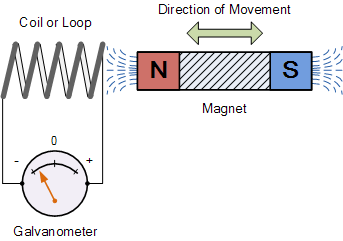
\includegraphics{electromagnetism-mag22.png}
    \caption{experiment of faraday}
    \label{fig:enter-label}
\end{figure}

\paragraph{Michael Faraday discovered this law of electromagnetic induction. He set up a lead wire according to the diagram above, which he connected to a device that measured the voltage across the circuit. When a bar magnet passes through the snaking, the voltage in the circuit is measured. The significance of this is that it is a method of producing electrical energy in a circuit by using magnetic fields rather than batteries. Machines such as generators, transformers, and motors operate on the principle of electromagnetic induction.~\cite{hcverma1992conceptsofphysics}}

\bibliography{refs}
\bibliographystyle{alpha}

\end{document}
